%%%%%%%%%%%%%%%%%%%%%%%%%%%%%%%%%%%%%%%%%%%%%%%%
%% Compile the master file!
%% 		Include: Antonio Machicao y Priemer
%% 		Course: GK Linguistik
%%%%%%%%%%%%%%%%%%%%%%%%%%%%%%%%%%%%%%%%%%%%%%%%


%%%%%%%%%%%%%%%%%%%%%%%%%%%%%%%%%%%%%%%%%%%%%%%%%%%%
%%%             Metadata                         
%%%%%%%%%%%%%%%%%%%%%%%%%%%%%%%%%%%%%%%%%%%%%%%%%%%%      

\title{Grundkurs Linguistik}

\subtitle{Morphologie II: Wortbildung \& Komposition}

\author[A. Machicao y Priemer]{
	{\small Antonio Machicao y Priemer}
	\\
	{\footnotesize \url{http://www.linguistik.hu-berlin.de/staff/amyp}}
	%	\\
	%	{\small\href{mailto:mapriema@hu-berlin.de}{mapriema@hu-berlin.de}}
}

\institute{Institut für deutsche Sprache und Linguistik}

% bitte lassen, sonst kann man nicht sehen, von wann die PDF-Datei ist.
%\date{ }

%\publishers{\textbf{6. linguistischer Methodenworkshop \\ Humboldt-Universität zu Berlin}}

%\hyphenation{nobreak}

%%@ee ggf. zusätzl. Übungen in: 2012-2013 WS MyP Doering/04. Morphologie/02c ÜB........ FALLS NICHT SCHON IM TUTORIUM VERWENDET!?
%%%%%%%%%%%%%%%%%%%%%%%%%%%%%%%%%%%%%%%%%%%%%%%%%%%%
%%%             Preamble's End                  
%%%%%%%%%%%%%%%%%%%%%%%%%%%%%%%%%%%%%%%%%%%%%%%%%%%%      


%%%%%%%%%%%%%%%%%%%%%%%%%
\huberlintitlepage
\iftoggle{toc}{
	\frame{
		%\begin{multicols}{2}
		\frametitle{Inhaltsverzeichnis}
		\tableofcontents
		%[pausesections]
		%\end{multicols}
	}
}

%%%%%%%%%%%%%%%%%%%%%%%%%%%%%%%%%%
%%%%%%%%%%%%%%%%%%%%%%%%%%%%%%%%%%
%%%%%LITERATURE:

%% Allgemein
\nocite{Glueck&Roedel16a}
\nocite{Schierholz&Co18}
\nocite{Luedeling2009a}
\nocite{Meibauer&Co07a} 
\nocite{Repp&Co15a} 

%%% Sprache & Sprachwissenschaft
%\nocite{Fries16c} %Adäquatheit
%\nocite{Fries16a} %Grammatikalität
%\nocite{Fries&MyP16c} %GG
%\nocite{Fries&MyP16b} %Akzeptabilität
%\nocite{Fries&MyP16d} %Kompetenz vs. Performanz

%%% Phonetik & Phonologie
%\nocite{Altmann&Co07a}
%\nocite{DudenAussprache00a}
%\nocite{Hall00a} 
%\nocite{Kohler99a}
%\nocite{Krech&Co09a}
%\nocite{Pompino95a}
%\nocite{Ramers08a}
%\nocite{Ramers&Vater92a}
%\nocite{Rues&Co07a}
%\nocite{WieseR96a}
%\nocite{WieseR11a}

%%% Graphematik
%\nocite{Altmann&Co07a}
%\nocite{Duerscheid04a}
%\nocite{Eisenberg00a}
%\nocite{Fuhrhop08a}
%\nocite{Fuhrhop09a}
%\nocite{Fuhrhop&Co13a}

%% Morphologie
%\nocite{Bauer00a} %Word
\nocite{Eisenberg00a}
\nocite{Fleischer00a} %Wortbildungsprozesse
\nocite{Fleischer&Barz12a} %Einführung Morphologie
\nocite{Fries&MyP16j} %Kopf
\nocite{Fuhrhop96a} %Fugenelemente
\nocite{Fuhrhop00a} %Fugenelemente
\nocite{Grewendorf&Co91a} %Betonung bei Komposita
\nocite{Haspelmath2002a}
\nocite{MyP18b} %Kopf
\nocite{Olsen86a} %Morphologie des Deutschen
\nocite{Olsen14a} %Coordinative Structures
%\nocite{Plungian00a} %Morphologie im Sprachsystem
%\nocite{Salmon00a} %Term Morphology
\nocite{Wegener03b} %Fugenelemente
\nocite{Wurzel00a} %Gegenstand Morphologie
\nocite{Wurzel00b} %Wort


%%%%%%%%%%%%%%%%%%%%%%%%%%%%%%%%%%%
%%%%%%%%%%%%%%%%%%%%%%%%%%%%%%%%%%%
\section{Morphologie II}
%%%%%%%%%%%%%%%%%%%%%%%%%%%%%%%%%%%

\begin{frame}
\frametitle{Begleitlektüre}

\begin{itemize}
	\item \textbf{obligatorisch:}
	\item[] \citet[41--45]{Abramowski2016a}
	\item \textbf{optional:}
	\item[] \citet[Kap. 2, S. 29--36]{Meibauer&Co07a}
	
\end{itemize}

\end{frame}


%%%%%%%%%%%%%%%%%%%%%%%%%%%%%%%%%%
%%%%%%%%%%%%%%%%%%%%%%%%%%%%%%%%%%
\subsection{Einführung}

\iftoggle{sectoc}{
	\frame{
		%		\begin{multicols}{2}
		\frametitle{~}
		\tableofcontents[currentsubsection,subsubsectionstyle=hide]
		%		\end{multicols}
	}
}

%%%%%%%%%%%%%%%%%%%%%%%%%%%%%%%%%%
\begin{frame}
\frametitle{Einführung}

\begin{itemize}
	\item \textbf{Wortschatz des Deutschen}: 5,3 Mio.\ Wörter
	
	\ras keine \textbf{Sprachverarmung}!
	
	\item \textbf{verschiedene Zählungen}: 300\,000--500\,000 Wörter und Phraseologismen 
	
	abhängig von \textbf{fachlichen} und \textbf{regionalen Wortschätzen}, von \textbf{veralteten} und \textbf{neuen} Wörtern, darüberhinaus: wann ist ein Wort \textbf{ein Wort} und wann \textbf{zwei Wörter}?
	
\medskip 
\pause 
	
	\item Duden:
	\begin{itemize}
		\item Urduden (1880): 27 000 Stichwörter
		\item Duden 26.\ Aufl. (2013): 140 000 Stichwörter
		\item Duden 27.\ Aufl. (2017): 145 000 Stichwörter
	\end{itemize}	
	
	\item Oxford Dictionary of English: 620\,000 Stichwörter
	\item Grand Robert: 100\,000 Stichwörter
	
\medskip 
\pause 
	
	\item durchschnittlicher \textbf{aktiver Wortschatz} im Deutschen:
	10\,000--20\,000 Wörter
	
\end{itemize}

\end{frame}


%%%%%%%%%%%%%%%%%%%%%%%%%%%%%%%%%%

\begin{frame}
\frametitle{Einführung}


\begin{quote}
``Der deutsche Wortschatz hat im Verlauf des 20. Jahrhunderts um etwa ein Drittel (\dots ) zugenommen'' (W. Klein). Die weitaus meisten neuen Wörter sind Ableitungen (wie \gqq{\emph{Zocker}} von \gqq{\emph{zocken}}) oder Zusammensetzungen (wie \gqq{\emph{Endlösung}}).
\end{quote}
\hfill \citep{Heine14a}

\medskip 

\begin{itemize}
\item Jährlich werden ung.\ \textbf{1\,000 neue Wörter} in den Duden aufgenommen \\
(5\,000 im Jahr 2018), davon ung.:

\begin{itemize}
	\item 83\% \textbf{Wortbildungen} (\zB \emph{facebooken}, \emph{gegenchecken}, \emph{entfreunden}, \emph{Späti})
	\item 12\% neue Bedeutung alter Wörter (\zB \emph{runterwürgen}, \emph{verpeilen})
	\item 5\% Entlehnungen (\zB \emph{tindern}, \emph{liken})
	\item außerdem: neue Redewendungen (\zB \emph{Es ist alles im grünen Bereich})
\end{itemize}

\end{itemize}

\end{frame}


%%%%%%%%%%%%%%%%%%%%%%%%%%%%%%%%%%
\begin{frame}
\frametitle{Einführung (zur Erinnerung)}

Die Morphologie unterteilt man in:
	
	\begin{itemize}
		\item \textbf{Wortbildung:} Ableitung und Zusammensetzung lexikalischer Wörter:
		
		\eal 
			\ex {[anforder(n)] $+$ [-ung] $=$ \alertred{Anforderung}}
			\ex {[les(e)] $+$ [kreis] $=$ \alertred{Lesekreis}}
		\zl
		
		\item \textbf{Wortformenbildung} (Flexion): Bildung von Wortformen in einem Paradigma: 
		
		\begin{itemize}
			\item Deklination der Nomina: 
			
			\ea (der) Lesekreis, (den) Lesekreis, (dem) Lesekreis(e), (des) Lesekreises, \ldots
			\z 
			
			\item Konjugation der Verben: 
			
			\ea fordere, forderst, fordert, fordern, \ldots 
			\z 
		\end{itemize}	
	\end{itemize}	

\end{frame}


%%%%%%%%%%%%%%%%%%%%%%%%%%%%%%%%%%%
\begin{frame}
\frametitle{Einführung (zur Erinnerung)}

\begin{itemize}
	\item \textbf{Wortbildung}
	
	\begin{itemize}
		\item neue lexikalische Wörter
		\item neue lexikalische Bedeutung (Begriffe)
		\item Ausgangswörter können einfache (Simplizia) oder komplexe Lexeme sein.
		\item Änderung der Wortart ist möglich (vgl.\ (\ref{ex:5bWortart1})) aber nicht zwingend (vgl.\ (\ref{ex:5bWortart2})). 
		
		\ea\label{ex:5bWortart1} {[\MyPdown{V}bearbeit] $+$ -ung $=$ [\MyPdown{N}Bearbeitung]}
		\ex\label{ex:5bWortart2} {be- $+$ [\MyPdown{V}arbeit](-en) $=$ [\MyPdown{V}bearbeit](-en)}
		\z
	\end{itemize}

	\item \textbf{Flexion}
	
	\begin{itemize}
		\item Flexionsmorpheme sind \textbf{rechtsperipher}: sie werden \textbf{erst nach der Wortbildung} mit dem Stamm verbunden
		\item Flexionsmorpheme enthalten nicht zwingend einen Vokal (nur Schwa):
		
		\ea Wortbildungsaffixe: \emph{-ung}, \emph{-in}, \emph{-bar}, \emph{ent-}, \ldots 
		\ex Flexionsaffixe: \emph{-en}, \emph{-t}, \emph{-est}, \emph{-st}, \emph{-n}, \emph{ge- -t}, \ldots 
		\z
		
	\end{itemize}
\end{itemize}

\end{frame}


%%%%%%%%%%%%%%%%%%%%%%%%%%%%%%%%%%
%%%%%%%%%%%%%%%%%%%%%%%%%%%%%%%%%%
\subsection{Struktur komplexer Wörter}

\iftoggle{sectoc}{
	\frame{
		%		\begin{multicols}{2}
		\frametitle{~}
		\tableofcontents[currentsubsection,subsubsectionstyle=hide]
		%		\end{multicols}
	}
}

%%%%%%%%%%%%%%%%%%%%%%%%%%%%%%%%%%

\begin{frame}
\frametitle{Struktur komplexer Wörter}

\begin{itemize}
		\item Die meisten Wortbildungsprozesse sind \textbf{konkatenativ} (vgl.\ (\ref{ex:5bKonk1}) \vs (\ref{ex:5bKonk2})).
	
	\settowidth\jamwidth{[ nicht konkatenativ]} 
	\ea\label{ex:5bKonk1} {[\MyPdown{N}Tisch] $+$ [\MyPdown{N}bein] \ras [\MyPdown{N}Tischbein]} 
	\jambox{[konkatenativ]}
	
	\ex\label{ex:5bKonk2} {[\MyPdown{V}schlaf] \ras [\MyPdown{N}Schlaf]}
	\jambox{[nicht konkatenativ]}
	\z 
	
\end{itemize}

\medskip 

\begin{block}{Konkatenation (auch Verkettung)}
	Prozess und Ergebnis einer systematischen linearen \textbf{Aneinanderreihung} linguistischer Kategorien	\citep[vgl.][]{Fries16i, Fuhrhop17a} 
\end{block}	


\end{frame}


%%%%%%%%%%%%%%%%%%%%%%%%%%%%%%%%%%
\begin{frame}
\frametitle{Struktur komplexer Wörter}

\begin{minipage}{.65\textwidth}

	\begin{itemize}
		\item Die Wortstruktur spiegelt \textbf{Bildungsprozess} wider.
		\item Sie steuert die \textbf{Interpretation}.
		\item In den meisten Theorien ist die komplexe Struktur \textbf{binär}.
		
		\begin{itemize}
			\item \textbf{Maximal} zwei Elemente ($=$ \textbf{Konstituenten} von engl. \emph{constituent} \gq{Bestandteil}) verbinden sich zu einem komplexen Element.
			\item Zwei Elemente gehören enger zusammen.
		\end{itemize}
		\item Aufbau ist \textbf{hierarchisch} \\
		(vgl.\ phonologische Struktur)
	\end{itemize}

\end{minipage}
%
\hfill%
%
\begin{minipage}{.34\textwidth}
\begin{figure}	
\centering
\scalebox{0.7}{
\begin{forest} 
	[Haustürschlüssel
		[Haustür
			[Haus] 
			[Tür]]
		[Schlüssel]]									
\end{forest}}

\vspace{.75cm}

\scalebox{.7}{
\begin{forest}
	[Zugverbindung
		[Zug]
		[Verbindung
			[verbind
				[ver-]
				[bind]]
			[-ung]]]
\end{forest}}
\end{figure}
\end{minipage}

\end{frame}


%%%%%%%%%%%%%%%%%%%%%%%%%%%%%%%%%%
\begin{frame}
\frametitle{Struktur komplexer Wörter}

\begin{minipage}{0.65\textwidth}
\begin{itemize}
	\item Morphologische Einheiten (Stämme, Basen, Affixe) sind \textbf{kategoriell ausgezeichnet}, \dash es wird markiert, ob es sich bspw. 
	
	\begin{itemize}
		\item um Nomenstämme (\alertred{N}), Verbstämme (\alertred{V}), \ldots 
		\item[] bzw.
		\item um Nomenaffixe (\alertblue{N\MyPup{af}}), Verbaffixe (\alertblue{V\MyPup{af}}), \ldots\  handelt
	\end{itemize}
\end{itemize}
\end{minipage}
%
\hfill%
%
\begin{minipage}{.34\textwidth}

\begin{figure}	
\centering
\scalebox{0.7}{
\begin{forest} 
sm edges,
	[\alertred{N}
		[\alertred{N}
			[\alertred{N}
				[Haus]]
			[\alertred{N} 
				[Tür]]]
		[\alertred{N}
			[Schlüssel]]]								
\end{forest}}

\vspace{.5cm}

\centering
\scalebox{.7}{
\begin{forest}
sm edges,
	[N
		[N		
			[Zug]]
		[N
			[V				
				[\alertblue{V\MyPup{af}}					
					[ver-]]
				[V
					[bind]]]
			[\alertblue{N\MyPup{af}}			
				[ung]]]]
\end{forest}}
\end{figure}
\end{minipage}
\end{frame}


%%%%%%%%%%%%%%%%%%%%%%%%%%%%%%%%%%
\begin{frame}
\frametitle{Struktur komplexer Wörter}

\begin{minipage}{.66\textwidth}

\begin{itemize}
	
	\item Die einzelnen Elemente haben \textbf{Beschränkungen}, mit welchen anderen Elementen sie sich verbinden können.

\pause 
	
	\item Ein \textbf{Präfix} der Kategorie $\alertred{X}$\MyPup{af} kann sich nur mit Elementen der Kategorie $\alertred{X}$ verbinden.

	\ea[*]{
		[\MyPdown{V\MyPup{af}}ver-] $+$ [\MyPdown{N}bindung] $=$ \alertred{\ding{56}} verbindung
	}
	\ex[]{
		[\MyPdown{V\MyPup{af}}ver-] $+$ [\MyPdown{V}bind] $=$ \alertred{\ding{52}} verbind 
	}
	\z 	

%\pause 
	
	\item Ein \textbf{Suffix} der Kategorie $\alertred{X}$\MyPup{af} bestimmt, mit welchen Elementen (\zB $X$, $Y$, $Z$) es sich verbinden kann.
	
	\ea {\alertred{\ding{52}} [\MyPdown{V}bind]$+$[\MyPdown{N\MyPup{af}}-ung], \alertred{\ding{56}} [\MyPdown{N}Lampe]$+$[\MyPdown{N\MyPup{af}}-ung]}
	\z 
\end{itemize}

\end{minipage}
%
\hfill%
%
\begin{minipage}{.32\textwidth}

\begin{figure}	
\centering
\scalebox{.7}{
\begin{forest}
sm edges,
	[\alertred{*}N
		[N
			[Zug]]
		[\alertred{*}N
			[V\MyPup{af}
				[ver-]]
			[N
				[V
					[bind]]
				[N\MyPup{af}
					[-ung]]]]]
\end{forest}}
\caption{ungrammatische Struktur}
\end{figure}

\end{minipage}
\end{frame}


%%%%%%%%%%%%%%%%%%%%%%%%%%%%%%%%%%
\begin{frame}
\frametitle{Struktur komplexer Wörter: Kopf}


\begin{itemize}
	\item Das \textbf{rechte Element} in (\ref{ex:5bKonk3}) und (\ref{ex:5bKonk4}) bestimmt die \textbf{Kategorie} des Wortbildungsprodukts %,MyP18b}
	
\ea 
	\ea\label{ex:5bKonk3} {[\MyPdown{V}brauch] $+$ [\MyPdown{\alertred{A\MyPup{af}}}-bar] $=$ [\alertred{\MyPdown{A}}brauchbar]}
	\ex\label{ex:5bKonk4} {[\MyPdown{A}brauchbar] $+$ [\MyPdown{\alertred{N\MyPup{af}}}-keit] $=$ [\alertred{\MyPdown{N}}Brauchbarkeit]}
	\z 
\z 

\end{itemize}

\pause 
	
\begin{block}{Kopf}
	Element in einem \textbf{konkatenativen morphosyntaktischen Prozess}, das die \textbf{wichtigsten Eigenschaften} des Resultats bestimmt

\end{block}	

\pause 

\begin{block}{Kopfprinzip}
	\textbf{Jedes} komplexe Wort, das durch \textbf{Komposition} oder \textbf{Derivation} entstanden ist, hat einen morphologischen Kopf.
\end{block}	

\hfill (vgl.\ \citealp[76]{Olsen86a}; \citealp[]{MyP18b})
	
\end{frame}


%%%%%%%%%%%%%%%%%%%%%%%%%%%%%%%%%%
\begin{frame}
\frametitle{Struktur komplexer Wörter: Kopf}

\begin{minipage}{.7\textwidth}


\begin{itemize}
	\item In der \textbf{Wortbildung} legt der Kopf die \textbf{morphosyntaktischen} Eigenschaften des komplexen Wortes fest (\zB Genus, Wortart, Flexionsart, \ldots ). 

\medskip
 	
	\item Auch einige der \textbf{semantischen} Eigenschaften des Resultats werden vom Kopf bestimmt.

\medskip
	
	\item \textbf{Projektion:} Vom Kopf werden die Merkmale auf den sog. Mutterknoten übertragen.  

\medskip
	
	\item problematische Fälle:
		
		\ea verholz(-en), befreund(-en), beruhig(-en), Wasserablauf
		\z
		
%	\item[] \textbf{ÜB.2}
\end{itemize}


%\begin{block}{Righthand Head Rule}
%	die \textbf{am weitesten rechts stehende Konstituente} in einem \textbf{Wortbildungsprozess} ist der Kopf.
%\end{block}	

\end{minipage}
%
\hfill%
%
\begin{minipage}{.29\textwidth}

\begin{figure}	
	\centering
	\scalebox{.6}{
	\begin{forest}
		[N\\
		{[}\alertred{neut}{]}, name=N3K
		[N\\
		{[}\alertblue{mask}{]}, name=N2K
		[N\\	
		{[}fem{]}, name=N1
		[Kartoffel\\
		]
		]
		[N\\
		{[}\alertblue{mask}{]}, name=N2
		[salat\\
		]
		]	
		]
		[N\\
		{[}\alertred{neut}{]}, name=N3	
		[rezept\\
		]
		]
		]{
			\draw[->,dashed] (N2) to[out=east,in=east] (N2K);
			\draw[->,dashed] (N3) to[out=east,in=east] (N3K);
		}
	\end{forest}
}

\vspace{.5cm}

	\centering
	\scalebox{.6}{
\begin{forest}
	[\alertred{N}, name=N1
	[N\MyPup{af}, name=N0
	[un-]		
	]
	[\alertred{N}, name=A1
	[\alertblue{A}, name=V1 
	[V
	[brauch-]
	]
	[\alertblue{A}\MyPup{af}, name=V0
	[-bar]
	]
	]
	[\alertred{N}\MyPup{af}, name=A0
	[-keit]
	]
	]
	]{
		\draw[->,dashed] (V0) to[out=east,in=east] (V1);
		\draw[->,dashed] (A0) to[out=east,in=east] (A1);
		\draw[->,dashed] (A1) to[out=east,in=east] (N1);
	}
\end{forest}

}
\end{figure}

\end{minipage}

\end{frame}


%%%%%%%%%%%%%%%%%%%%%%%%%%%%%%%%%%
\begin{frame}
\frametitle{Struktur komplexer Wörter: Kopf}


\begin{minipage}{.49\textwidth}

	\centering
	\scalebox{.7}{
		\begin{forest}
			[N\\
			{[}\alertred{neut}{]}, name=N3K
			[N\\
			{[}\alertblue{mask}{]}, name=N2K
			[N\\	
			{[}fem{]}, name=N1
			[Kartoffel\\
			]
			]
			[N\\
			{[}\alertblue{mask}{]}, name=N2
			[salat\\
			]
			]	
			]
			[N\\
			{[}\alertred{neut}{]}, name=N3	
			[rezept\\
			]
			]
			]{
				\draw[->,dashed] (N2) to[out=east,in=east] (N2K);
				\draw[->,dashed] (N3) to[out=east,in=east] (N3K);
			}
		\end{forest}
	}

\end{minipage}
%
\hfill%
%	
\begin{minipage}{.49\textwidth}
	
	\centering
	\scalebox{.7}{
		\begin{forest}
			[\alertred{N}, name=N1
			[N\MyPup{af}, name=N0
			[un-]		
			]
			[\alertred{N}, name=A1
			[\alertblue{A}, name=V1 
			[V
			[brauch-]
			]
			[\alertblue{A}\MyPup{af}, name=V0
			[-bar]
			]
			]
			[\alertred{N}\MyPup{af}, name=A0
			[-keit]
			]
			]
			]{
				\draw[->,dashed] (V0) to[out=east,in=east] (V1);
				\draw[->,dashed] (A0) to[out=east,in=east] (A1);
				\draw[->,dashed] (A1) to[out=east,in=east] (N1);
			}
		\end{forest}
		
	}

\end{minipage}	

\bigskip 

\begin{block}{Righthand Head Rule (Rechstköpfigkeitsprinzip)}
	die \textbf{am weitesten rechts stehende Konstituente} in einem \textbf{Wortbildungsprozess} ist der Kopf.
\end{block}	

\end{frame}


%%%%%%%%%%%%%%%%%%%%%%%%%%%%%%%%%%
\begin{frame}
\frametitle{Struktur komplexer Wörter: Rekursion}


\begin{block}{Rekursion}
	Prozess, der es erlaubt, mittels einer \textbf{endlichen Menge von Elementen und Regeln} eine \textbf{unendliche Menge von Symbolfolgen} zu erzeugen\\
	\hfill  \citep[vgl.][]{Hetland14a, Olsen15a}. 
\end{block}

\begin{itemize}
	\item Durch rekursive Regeln (vgl.\ (\ref{ex:5bRekRegel1}) \& (\ref{ex:5bRekRegel2})) kann man eine unendliche Menge von Wörtern (oder Sätze) generieren.

	\item \textbf{Einige Wortbildungsprozesse} können rekursiv sein.
		
	\item Durch \textbf{Nominalkomposition} kann man sehr komplexe Stämme erzeugen (\ref{ex:5bRekRegel3}).
	
\end{itemize}

\settowidth\jamwidth{[XXabstrakte rekursive Regel]} 
\ea 
	\ea\label{ex:5bRekRegel1} $X \rightarrow Y~Z$, wobei $X = Y$ oder $X = Z$ 
	\jambox{[abstrakte rekursive Regel]}
	
	\ex\label{ex:5bRekRegel2} N \ras N N 
	\jambox{[konkrete rekursive Regel]}
		
	\ex\label{ex:5bRekRegel3} Rindfleischetikettierungsüberwachungsaufgabenübertragungsgesetz
	
	% SM: Gasherdverkäuferschulungszentrumseinrichtungsbudget
	\z 
\z 
\end{frame}


%%%%%%%%%%%%%%%%%%%%%%%%%%%%%%%%%%
\begin{frame}
\frametitle{Struktur komplexer Wörter: Rekursion}

\begin{minipage}{.74\textwidth}

\begin{itemize}
	\item Anwendung einer rekursiven Regel (\ref{ex:5bRekRegel4})
	
	\ea \label{ex:5bRekRegel4} $\alertblue{X} \rightarrow \alertblue{X}~Y$	
	\z 
	
	\item Mit einigen Affixen ist rekursive Wortbildung möglich:
	
	\ea \alertred{Ur}großmutter, \alertred{Ur}urgroßmutter, \alertred{Ur}ururgroßmutter, \ldots
	\z 
	
	\item Andere Affixe erlauben keine rekursive Wortbildung:
	\ea 
		\ea[]{Schönheit}
		\ex[*]{Schönheit\alertred{heit}}
		\z 
	\z 
	
\end{itemize}

\end{minipage}
%%
%%
\begin{minipage}[c]{.25\textwidth}

\begin{figure}
	\centering
	\scalebox{.9}{
		\begin{forest}
			[X
				[X
					[X
						[X]
						[Y]
					]
					[Y]
				]
				[Y]
			]	
		\end{forest}	
	}
\end{figure}

\end{minipage}

\end{frame}


%%%%%%%%%%%%%%%%%%%%%%%%%%%%%%%%%%
\begin{frame}
\frametitle{Struktur komplexer Wörter: Rekursion}

\begin{itemize}
	\item Mit Adjektiven als Erstglied ist \textbf{keine Rekursion} möglich.
	
	\ea *Samtigrotwein, *Weißmagerquark, *Feuchtgrünfutter
	\z
	
	\item Das kann in der Regel dadurch erfasst werden, dass die \textbf{Symbole rechts und links der Regel unterschiedlich} sind.
	
	\ea N\MyPdown{\alertred{1}} \ras A N\MyPdown{\alertred{2}}
	\z   
	
	\item Es gibt Ausnahmen:
	
	\ea Frühneuhochdeutsch, Billigrotwein
	\z 
	
\end{itemize}

\end{frame}


%%%%%%%%%%%%%%%%%%%%%%%%%%%%%%%%%%
%%%%%%%%%%%%%%%%%%%%%%%%%%%%%%%%%%
\subsection{Komposition}

\iftoggle{sectoc}{
	\frame{
		%		\begin{multicols}{2}
		\frametitle{~}
		\tableofcontents[currentsubsection,subsubsectionstyle=hide]
		%		\end{multicols}
	}
}

%%%%%%%%%%%%%%%%%%%%%%%%%%%%%%%%%%

\begin{frame}
\frametitle{Komposition}

\begin{itemize}
	\item Wortbildungsprozess mittels \textbf{Konkatenation}, bei dem zwei \textbf{Stämme} (Kompositionsglieder) zu einem neuen Stamm verbunden werden.
	
	\item Ergebnis der Komposition: \textbf{Kompositum} (Pl. Komposita)
	
	\item Jedes Kompositionsglied kann selbst auch morphologisch komplex (\zB ein Kompositum) sein.
	
	\ea
	\glll \alertred{Haustür} $\rightarrow$ Haus $+$ Tür \\
	Haustürschlüssel $\rightarrow$ {\alertred{[Haus$+$Tür]}} $+$ Schlüssel\\
	\textbf{Kompositum} {} \textbf{Erstglied} {} \textbf{Zweitglied} \\
	\z
	
\end{itemize}

\end{frame}


%%%%%%%%%%%%%%%%%%%%%%%%%%%%%%%%%%

\begin{frame}
\frametitle{Kopf des Kompositums}

\begin{itemize}
\item \textbf{Köpfigkeit:} rechtsperiphär

\item Ist das rechte Kompositionsglied ein Substantivstamm so ist das ganze Kompositum ein Substantiv.

\ea 
\ea wein\alertred{rot} -- Rot\alertred{wein}

\ex Karten\alertred{telefon} -- Telefon\alertred{karte}

\ex Fahr\alertred{rad} -- rad\alertred{fahr-}
\z
\z 

\end{itemize}

\begin{minipage}[t]{0.32\textwidth}
\centering
%		\scalebox{0.7}{
\begin{forest}
	[\alertred{A}
	[N
	[welt]]
	[\alertred{A}
	[fremd]]]
\end{forest}%}
\end{minipage}
%
%
\begin{minipage}[t]{0.32\textwidth}
\centering
%		\scalebox{0.7}{
\begin{forest}
	[\alertred{N}
	[A
	[klein]]
	[\alertred{N}
	[holz]]
	]
\end{forest}%}
\end{minipage}
%
%
\begin{minipage}[t]{0.34\textwidth}
\centering
%		\scalebox{0.7}{
\begin{forest}
	[\alertred{N}
	[\alertblue{V}
	[N
	[rad]
	]
	[\alertblue{V}
	[fahr]
	]
	]
	[\alertred{N}
	[weg]
	]
	]
\end{forest}
%	}
\end{minipage}

\end{frame}


%%%%%%%%%%%%%%%%%%%%%%%%%%%%%%%%%%
\begin{frame}
%\frametitle{Kopf}

\begin{itemize}
\item Der Kopf gibt nicht nur \textbf{kategorielle} sondern auch andere Merkmale an die Gesamtstruktur weiter.
\item Bei Nominalkomposita bestimmt der Kopf bspw. auch \textbf{Genus} und \textbf{Flexionsklasse}:

\eal 
\ex \alertred{der} Kartoffel\alertred{salat} -- \alertblue{die} Salat\alertblue{kartoffel}
\ex \alertred{die} Eis\alertred{schokolade} -- \alertblue{das} Schokoladen\alertblue{eis}
\ex die Kartoffelsalat + \alertred{-e} -- die Salatkartoffel + \alertblue{-n}

\zl

\end{itemize}
\end{frame}


%%%%%%%%%%%%%%%%%%%%%%%%%%%%%%%%%%
%%%%%%%%%%%%%%%%%%%%%%%%%%%%%%%%%%
\subsubsection{Fugenelemente}
\iftoggle{toc}{
	\frame{
		\begin{multicols}{2}
			\frametitle{~}
			\tableofcontents[currentsection]
		\end{multicols}
	}
}
%%%%%%%%%%%%%%%%%%%%%%%%%%%%%%%%%%

\begin{frame}
\frametitle{Fugenelemente}

\begin{itemize}
	\item Komposition ist nicht immer einfach die Konkatenation von Stämmen.
	
	\item In ung. 30\% der Kompositionen wird noch etwas \textbf{hinzugefügt}, manchmal wird etwas \textbf{getilgt} (vgl.\ (\ref{ex:5bSchwaTilg})).
	
	\settowidth\jamwidth{[XSchwa-Tilgung]} 
	\eal 
		\ex %\emph{-es}-Einsetzung: \\
		 {[\MyPdown{N}Land\alertred{es}hauptstadt]\ra [\MyPdown{N}Land]$+$\alertred{-es}$+$[\MyPdown{N}Hauptstadt]}
		 \jambox{[\emph{-es}-Einsetzung]}
		 
		\ex %\emph{-e}-Einsetzung: \\
		 {[\MyPdown{N}Hund\alertred{e}futter]\ra [\MyPdown{N}Hund]$+$\alertred{-e}$+$[\MyPdown{N}Futter]}
		 \jambox{[\emph{-e}-Einsetzung]}
		 
		\ex %\emph{-s}-Einsetzung: \\
		 {[\MyPdown{N}Leitung\alertred{s}wasser]\ra [\MyPdown{N}Leitung]$+$\alertred{-s}$+$[\MyPdown{N}Wasser]}
		 \jambox{[\emph{-s}-Einsetzung]}
		 
		\ex\label{ex:5bSchwaTilg} %Schwa-Tilgung: \\
		 {[\MyPdown{N}Sprach\alertred{\_}kurs]\ra [\MyPdown{N}Sprache]$-$\alertred{-e}$+$[\MyPdown{N}Kurs]}
		 \jambox{[Schwa-Tilgung]}
	\zl
		 
\pause

	\item \textbf{Fugenelemente} entwickelten sich \textbf{aus Flexionsendungen} des ersten Kompositionsglieds. Synchron haben sie jedoch \textbf{keine Flexionsfunktion mehr}.
	
	\item Die \textbf{subtraktive Fuge} (vgl.\ (\ref{ex:5bSchwaTilg}) \& (\ref{ex:5bSubstrFuge})) kann mit Flexion nicht erklärt werden.
	
	\eal \label{ex:5bSubstrFuge}
	\ex die Perl\alertblue{e} -- Perl\alertred{\_}wein, Perl\alertred{\_}zwiebel
	\ex die Woll\alertblue{e} -- Woll\alertred{\_}knäuel
%	\ex die Kehl\alertblue{e} -- Kehl\alertred{\_}kopf, Kehl\alertred{\_}laut
	\zl
	
\end{itemize}

\end{frame}


%%%%%%%%%%%%%%%%%%%%%%%%%%%%%%%%%%
\begin{frame}
\frametitle{Fugenelemente}

\begin{itemize}
	\item \gqq{Fugenelement} impliziert, dass die hinzugefügten Elemente wie Fugen \textbf{zwischen} den beteiligten Stämmen stehen. 
	
\medskip 
	
	Das ist aus zwei Gründen problematisch:

	\begin{itemize}
		\item Die \textbf{Tilgung} (eine \gqq{negative Fuge}) kann so nicht erklärt werden.
		\item Es gibt Evidenz dafür, dass die hinzugefügten Elemente \textbf{zum Erstglied gehören} (\dash \textbf{keine trinäre Struktur}):

\pause 

\medskip 
	
	\begin{itemize}
		\item Sie bleiben bei \textbf{Koordinationsellipsen} (Weglassungen) beim Erstglied:
		
		\ea Leitung\alertred{s}- und Mineral\alertred{\_}wasser (nicht: \emph{und Mineral\alertred{s}wasser})
		\z

\pause 
		
		\item Wird das \textbf{Erstglied getilgt}, darf die Fuge nicht erhalten bleiben:
		
		\ea Kind\alertred{er}wagen und -sitz (nicht: \emph{und \alertred{-er}sitz})
		\z

\pause 
		
		\item Sie werden in der Regel \textbf{vom Erstglied bestimmt}:
		
		\ea Kuh\alertred{\_}+stall -- *Küh\alertred{e}$+$stall \vs *Huhn\alertred{\_}$+$stall -- Hühn\alertred{er}$+$stall
		\z
		
		\ea aber: Rind\alertred{\_}$+$fleisch -- Rind\alertred{s}$+$leder -- Rind\alertred{er}$+$braten
		\z
		
	\end{itemize}

%	\item[] \textbf{ÜB.3}

\end{itemize}
\end{itemize}
\end{frame}


%%%%%%%%%%%%%%%%%%%%%%%%%%%%%%%%%%
\begin{frame}
\frametitle{Fugenelemente}

\begin{itemize}
	\item Die Flexionsendungen, die historisch zugrunde gelegen haben könnten, sind:
	
		\settowidth\jamwidth{[Xvorangestellte Genitivattribute]} 
		\ea Herz\alertred{ens}$+$angelegenheit, Land\alertred{es}$+$ministerium
		\jambox{[vorangestellte Genitivattribute]}

		\ex Häus\alertred{er}$+$front, Staat\alertred{en}$+$gemeinschaft
		\jambox{[Plural]}
		\z 

\pause 
	
	\item Es gibt jedoch zahlreiche \textbf{Gegenbeispiele}:
	
	\settowidth\jamwidth{[keine Genitivalternation bei Fuge]} 
	\eal 
		\ex Liebling\alertred{s}getränk \jambox{[semantisch falscher Genitiv]}
		\ex Lieb\alertred{es}brief \jambox{[formal falscher Genitiv]}
		\ex Hühn\alertred{er}ei, Scheib\alertred{en}wischer \jambox{[semantisch falscher Plural]}
		\ex Freund\alertred{es}kreis, Bischof\alertred{s}konferenz \jambox{[semantisch falscher Singular]}
		\ex Ende des Jahr\alertblue{es}/Jahr\alertblue{s} \jambox{[Genitivalternation]}
		
		\vs Jahr\alertred{es}zahl/*Jahr\alertred{s}zahl \jambox{[keine Genitivalternation bei Fuge]} 
	\zl
		 
\end{itemize}

\end{frame}


%%%%%%%%%%%%%%%%%%%%%%%%%%%%%%%%%%
\begin{frame}
\frametitle{Exkurs: Tendenzen für Fugenelemente}

\begin{itemize}
	\item Wortart des Erstglieds, Laut-, Silben- oder Wortbildungsstruktur 
	
	\item Es ist nicht möglich Fugenelemente 100\%ig vorherzusagen \citep[vgl.][]{Fuhrhop96a}.

\pause
	
	\item \textbf{phonologische Aspekte:}
	
	\begin{itemize}
		\item \textipa{[@]} nach stimmhaftem Konsonant im Stammauslaut bei verbalen Erstgliedern:
		
		\ea Pfleg-\alertred{e}-fall, Les-\alertred{e}-ecke (aber: Lesart), Reib-\alertred{e}-kuchen
		\z
		
		\item Aufeinanderfolge zweier betonter Silben wird verhindert\\
		(Primärakzent: \textprimstress / Sekundärakzent: \textsecstress):
		
		\ea \textprimstress Licht\alertred{\_}.re.\textsecstress kla.me vs. \textprimstress Lich.t\alertred{er}.\textsecstress ket.te (aber: \textprimstress Licht\alertred{\_}.\textsecstress schal.ter)
		\z
			
	\end{itemize}

\pause 

	\item \textbf{morphologische Aspekte:}
	
	\begin{itemize}
		\item \ab{-s} steht \emph{manchmal} nach komplexen Erstgliedern

		\ea {[[Hand$+$werk]\alertred{-s}]$+$[zeug] \vs [Werk]$+$[zeug] }
		\z 
	\end{itemize}

\end{itemize}

\end{frame}


%%%%%%%%%%%%%%%%%%%%%%%%%%%%%%%%%%
\begin{frame}
\frametitle{Fugenelement \vs Stammform}

\begin{itemize}
	\item Einige Autoren \citep[vgl.][211ff; 227ff]{Eisenberg00a} sprechen von \textbf{Kompositionsstammformen} (KS): nicht nur der Stamm eines Nomens \\
	(\zB \ab{kind}) ist \textbf{im Lexikon} verzeichnet, sondern auch die vorkommenden Kompositionsstammformen (vgl.\ (\ref{ex:5bKSFormen})).
	
	\item Lexikon als Speicher von \textbf{Idiosynkrasien}, \dash von Nicht-Derivierbarem
	
	\settowidth\jamwidth{XXXXXXXXXXXXXXXXXXXXXXXXXXXXXXXXXXX} 
	\ea\label{ex:5bKSFormen} \ab{kind}:\\
	KS\MyPdown{1}: kinder \jambox{\zB in \emph{Kind\alertred{er}wagen}} 
	
	KS\MyPdown{2}: kindes \jambox{\zB in \emph{Kind\alertred{es}entführung}} 
	
	KS\MyPdown{3}: kinds \jambox{\zB in \emph{Kind\alertred{s}kopf}}
	
	KS\MyPdown{4}: kind \jambox{\zB in \emph{Kind\alertred{\_}frau}}
	\z    
	
	\item Ähnlich werden bei der Derivation \textbf{Derivationsstammformen} angenommen:
	
	\ea hoffnung\alertred{s}-los, sag\alertred{e}n-haft, wein\alertred{er}-lich, Hütt\alertred{\_}-chen
	\z

\end{itemize}

\end{frame}


%%%%%%%%%%%%%%%%%%%%%%%%%%%%%%%%%%
\begin{frame}
\frametitle{Fugenelement \vs Stammform}

\begin{minipage}{.78\textwidth}
	
Struktur nach der \textbf{Annahme einer Kompositionsstammform}:

\begin{itemize}	
	\item Fugenelement ist \textbf{kein Morphem}.

	\item Fugenelement und Stamm bilden eine \textbf{untrennbare Einheit}.
	
	\item \ab{Kinder-} ist im Lexikon als Allomorph von \ab{Kind} verzeichnet.
	
	\item Annahme: Form \ab{Kinder-} ist \textbf{nicht vorhersagbar}.
\end{itemize}

\end{minipage}
%%
%%
\begin{minipage}{.21\textwidth}	
	\centering	
	\scalebox{.8}{
	\begin{forest}
		[N
		[N 
		[Kind\alertred{(-er)}]
		]
		[N
		[Wagen]
		]
		]	
	\end{forest}
	}
\end{minipage}

\begin{minipage}{.76\textwidth}

\pause 

\medskip 

Struktur nach der \textbf{Annahme eines Fugenelements:}

\begin{itemize}	
	\item Fugenelement ist \textbf{kein Morphem}.
	
	\item Fugenelement bildet mit Stamm eine \textbf{neue Konstituente}.
	
	\item \ab{Kind} ist im Lexikon verzeichnet, FE \ab{-er} wird durch eine \textbf{Regel} hinzugefügt.
	
	\item Annahme: Form \ab{Kinder} ist (irgendwie) \textbf{vorhersagbar}.
\end{itemize}
	
\end{minipage}
%%
%%
\begin{minipage}{.23\textwidth}	
	\centering	
	\scalebox{.8}{
	\begin{forest}
		%MyP edges,	
		[N
		[N 
		[Kind]
		[FE
		[\alertred{-er}]
		]
		]
		[N
		[Wagen]
		]
		]		
	\end{forest}
	}
\end{minipage}

\end{frame}


%%%%%%%%%%%%%%%%%%%%%%%%%%%%%%%%%%
%%%%%%%%%%%%%%%%%%%%%%%%%%%%%%%%%%
\subsubsection{Komposita: Funktionale Klassifikation}
%\iftoggle{sectoc}{
%	\frame{
%		\begin{multicols}{2}
%			\frametitle{~}
%			\tableofcontents[currentsection]
%		\end{multicols}
%	}
%}

%%%%%%%%%%%%%%%%%%%%%%%%%%%%%%%%%%

\begin{frame}
\frametitle{Komposita: Funktionale Klassifikation}

\begin{itemize}
	\item Komposita kann man nach der \textbf{semantischen Beziehung} \\
	zwischen \textbf{Erst-} und \textbf{Zweitglied} klassifizieren.
	
	\begin{block}{Determinativkompositum}
		Das Erstglied \textbf{bestimmt} das Zweitglied \textbf{näher}. 
	\end{block}
	
	\settowidth\jamwidth{XXXXXXXXXXXXXXXXXXXXXXXXXXXXXXXXXXX}

	\ea {[Wein$+$Flasche]} \jambox{$=$ \gq{$x$ ist eine Flasche, die etwas mit Wein zu tun hat.}}
	
	\jambox{$\neq$ \gq{$x$ ist eine Flasche und $x$ ist Wein.}}
	\z 

\pause 
	
	\begin{block}{Kopulativkompositum}
		Das Erstglied und das Zweitglied sind \textbf{gleichrangig}.\\
		Es ist nicht der Fall, dass das Erstglied  das Zweitglied \textbf{näher} \textbf{bestimmt}. 
	\end{block}
	
	\ea {[süß$+$sauer]} \jambox{$=$ \gq{$x$ ist süß und $x$ ist sauer}}
	\z 
	
\end{itemize}

\end{frame}


%%%%%%%%%%%%%%%%%%%%%%%%%%%%%%%%%%
%%%%%%%%%%%%%%%%%%%%%%%%%%%%%%%%%%
\subsubsubsection{Determinativkomposita}
%\iftoggle{sectoc}{
%	\frame{
%		\begin{multicols}{2}
%			\frametitle{~}
%			\tableofcontents[currentsection]
%		\end{multicols}
%	}
%}
%%%%%%%%%%%%%%%%%%%%%%%%%%%%%%%%%%%

\begin{frame}
\frametitle{Determinativkomposita}

\begin{itemize}
	\item \alertblue{Erste Konstituente} (auch: Bestimmendes/Determinans) bestimmt\\
	die \alertred{zweite Konstituente} (auch: Bestimmtes/Grundwort/Determinatum) näher.

	\item Das Kompositum bezeichnet eine \textbf{Unterart} des durch die \alertred{zweite Konstituente} Bezeichneten.

	\settowidth\jamwidth{XXXXXXXXXXXXXXXXXXXXXXXXXXXXX}
	\ea 
		\ea \alertblue{Wein}$+$\alertred{flasche} \jambox{\ras \alertred{Flasche}}
		\ex \alertblue{Flasche(-n)}$+$\alertred{Wein} \jambox{\ras \alertred{Wein}}
		\z
	
	\ex 
		\ea \alertblue{Stern(-en)}$+$\alertred{himmel} \jambox{\ras \alertred{Himmel}}
		\ex \alertblue{Himmel(-s)}$+$\alertred{stern} \jambox{\ras \alertred{Stern}}
		\z
	
	\ex 	
		\ea \alertblue{Fenster}$+$\alertred{glas} \jambox{\ras \alertred{Glas}}
		\ex \alertblue{Glas}$+$\alertred{fenster} \jambox{\ras \alertred{Fenster}}
		\z 
	\z
	
	\item produktivste Art der Komposition (ung.\ 80\% der Komposita)
\end{itemize}

\end{frame}


%%%%%%%%%%%%%%%%%%%%%%%%%%%%%%%%%%%
\begin{frame}
\frametitle{Determinativkomposita}


Bedeutungsbeziehung ist \textbf{vielfältig} und \textbf{nicht eindeutig bestimmbar}.

\begin{columns}
	
\column[t]{.5\textwidth}

\begin{itemize}

	\item \textbf{räumlich},  \textbf{zeitlich} oder \textbf{kausal}
	
	\ea Gartentor, Winterferien, Freudentränen
	\z
	
	\item \textbf{Konstitution} des Zweitglieds (bestehen aus, haben, Form/Farbe):
	
	\ea Holzkäfig, Kapuzenjacke, Grünspecht
	\z

	\item \textbf{Zweck} des Zweitglieds \\
	(dienen zu, schützen vor)

	\ea Haarband, Regenmantel
	\z	
\end{itemize}

\column[t]{.5\textwidth}
	
\begin{itemize}
	\item \textbf{Instrument}eigenschaft des Zweitglieds (funktioniert mit Hilfe von)
	
	\ea Benzinmotor, Windrad
	\z
	
	\item \textbf{Vergleich}sbeziehung
	
	\ea aalglatt, krebsrot
	\z
	
	\item \textbf{steigernde} Bedeutung
	
	\ea bitterernst, mordsgeil, bettelarm
	\z
\end{itemize}

\end{columns}
	
\end{frame}


%%%%%%%%%%%%%%%%%%%%%%%%%%%%%%%%%%
\begin{frame}
\frametitle{Determinativkomposita}
	
Es ist nicht immer klar, wie genau die Bedeutungsbeziehung zwischen Erst- und Zweitglied ist. Sie ist \textbf{unabhängig} von \textbf{grammatischen Faktoren} und hängt häufig vom \textbf{Weltwissen}, \textbf{Kontext}, usw. ab:
	
\settowidth\jamwidth{XXXXXXXXXXXXXXXXXXXXXXXXXXXXXXXXXXXXXXX}
	\ea Fischmann	\jambox{$=$ \gq{Mann, der Fisch verkauft}}
							\jambox{$=$ \gq{Mann, der wie ein Fisch aussieht}}
							\jambox{$=$ \gq{Mann, der nach Fisch riecht}}
							\jambox{$=$ \gq{Mann, der viel über Fische redet}}
							\jambox{\ldots}

\pause 
		
\settowidth\jamwidth{XX[Weltwissen, Kontext, etc.]}
	\ex Auf einem Werbeschild:
	
	Hühner-Kebap 2,50€\\
	Kinder-Kebap 1,10€ \jambox{[Weltwissen, Kontext, etc.]}
	\z
	
	%\begin{figure}
	%\centering
	%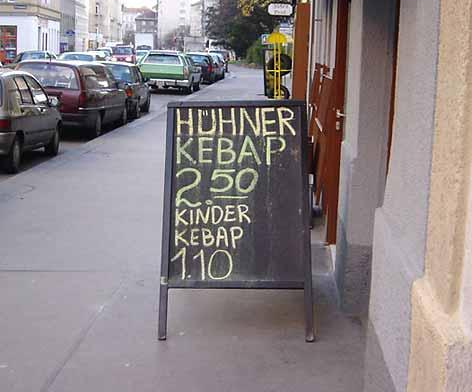
\includegraphics[scale=.55]{material/05Morph-Kebap}
	%\end{figure}
	
\end{frame}


%%%%%%%%%%%%%%%%%%%%%%%%%%%%%%%%%%
%%%%%%%%%%%%%%%%%%%%%%%%%%%%%%%%%%
\subsubsubsection{Rektionskomposita}
%\iftoggle{sectoc}{
%	\frame{
%		\begin{multicols}{2}
%			\frametitle{~}
%			\tableofcontents[currentsection]
%		\end{multicols}
%	}
%}
%%%%%%%%%%%%%%%%%%%%%%%%%%%%%%%%%%

\begin{frame}
\frametitle{Rektionskomposita}

\begin{itemize}
	\item wichtige \textbf{Untergruppe} der Determinativkomposita
	
	\ea Bus\alertred{fahrer} $=$ \gq{\alertred{Fahrer}, der einen Bus fährt}
	\z 
\end{itemize}

\pause 

\begin{block}{Rektion}
	Art der \textbf{syntagmatischen Beziehung} zwischen zwei Einheiten, bei der die eine \textbf{grammatische Eigenschaften} der anderen bestimmt. I.\,d.\,R. redet man von Rektion bei Verben, aber andere Wortarten regieren auch Argumente.  Verben bestimmen bspw.\ den Kasus ihrer Argumente (vgl.\ (\ref{ex:5bKasus2}) \vs (\ref{ex:5bKasus3})) 
	
	\hfill \citep[vgl.][]{McIntyre13a, MyP16e}.

\end{block}

\ea 
	\ea\label{ex:5bKasus2} {Jakob \textbf{unterstützt} [\MyPdown{\alertred{\textsc{akk}}}den Verein].}
	\ex\label{ex:5bKasus3} {Jakob \textbf{hilft} [\MyPdown{\alertred{\textsc{dat}}}dem Verein].}
	\z
\z  

\end{frame}


%%%%%%%%%%%%%%%%%%%%%%%%%%%%%%%%%%
\begin{frame}
\frametitle{Rektionskomposita}

\begin{itemize}
	\item Bedeutungsbeziehung zwischen Erst- und Zweitglied ist durch die \textbf{Argumentstruktur des Zweitglieds} bestimmt (vgl.\ (\ref{ex:5bFolien})), sie ist nicht so ambig wie bei anderen Determinativkomposita (vgl.\ (\ref{ex:5bFischMann})).
	
	\ea 
		\ea\label{ex:5bFischMann} Fisch\alertred{mann} $=$ \gq{Mann, der \textbf{irgendwas} mit Fisch zu tun hat}
		\ex\label{ex:5bFolien} Folien\alertred{bearbeitung} $=$ \gq{Bearbeitung der Folien}
		\z 	
	\z 
\end{itemize}

\begin{itemize}
	\item Häufig findet man Rektionskomposita bei \textbf{deverbalen} Nomina
	

	\ea 
		\ea tag(-en) \ras Tag$+$\alertred{-ung}
		\ex bearbeit(-en) \ras Bearbeit$+$\alertred{-ung}
		\ex fahr(-en) \ras Fahr$+$\alertred{-er}		
		\z 
	\z 
	
\end{itemize}


\end{frame}


%%%%%%%%%%%%%%%%%%%%%%%%%%%%%%%%%%
\begin{frame}
\frametitle{Rektionskomposita}

\begin{itemize}
	
	\item Verb bestimmt, mit wie vielen und mit welchen Argumenten es im Satz erscheint (vgl.\ (\ref{ex:5bBsp1}) \& (\ref{ex:5bBsp2})) (s.\ Rektion, Valenz, Subkategorisierungsrahmen).
	
	\settowidth\jamwidth{[2 ArgumenteX]} 
	\ea \label{ex:5bBsp1} 
		\ea {[\MyPdown{\alertred{\textsc{subj}}}Die \alertred{Linguisten}] \alertblue{tagen}.}
		\jambox{[1 Argument]}
		\ex die \alertblue{Tagung} der Linguisten 
		\ex \alertred{Linguisten}\alertblue{tagung}
		\z 

	\ex \label{ex:5bBsp2} 
		\ea {jemand \alertblue{bearbeitet} [\MyPdown{\alertred{\textsc{obj}}}die \alertred{Folien}].}
		\jambox{[2 Argumente]}
		\ex die \alertblue{Bearbeitung} der Folien
		\ex \alertred{Folien}\alertblue{bearbeitung}
		\z 
	\z
	
	\item \textbf{Erstglied} in einem deverbalen Rektionskompositum realisiert ein \textbf{Argument} des \textbf{Verbs}, das der zweiten Konstituente zugrunde liegt.
	
	\ea	 
		\ea jemand \alertblue{fährt} \alertred{Auto} \ras \alertred{Auto}\alertblue{fahrer}
		\ex jemand \alertblue{beobachtet} das \alertred{Wetter} \ras \alertred{Wetter}\alertblue{beobachter} 
		\ex das \alertred{Rotkehlchen} \alertblue{singt} \ras \alertred{Rotkehlchen}\alertblue{gesang}
		\z 
	\z
		 
\end{itemize}

\end{frame}


%%%%%%%%%%%%%%%%%%%%%%%%%%%%%%%%%%
\begin{frame}
\frametitle{Rektionskomposita}

\begin{itemize}
	\item Es gibt auch Rektionskomposita, bei denen die zweite Konstituente \textbf{nicht deverbal} ist, \zB Nomen oder Adjektiv.
	
	\settowidth\jamwidth{XXXXXXXXXXXXXXXXXXXXXX}
	\ea 
		\ea {[\MyPdown{N}\alertred{Angst} [\MyPdown{PP}vor der \alertblue{Prüfung}]]}
		\jambox{\ras \alertblue{Prüfungs}\alertred{angst}}

		\ex  {[\MyPdown{N}\alertred{Sehnsucht} [\MyPdown{PP}nach dem \alertblue{Tod}]]}
		\jambox{\ras \alertblue{Todes}\alertred{sehnsucht}}
		 
		\ex  {[[\MyPdown{DP}dem \alertblue{Staat}] \MyPdown{A}\alertred{treu}]}
		\jambox{\ras \alertblue{staats}\alertred{treu}}
		
		\ex {[\MyPdown{A}\alertred{sicher} [\MyPdown{PP}vor \alertblue{Fälschung}]]}
		\jambox{\ras \alertblue{fälschungs}\alertred{sicher}}
		
		\ex {[\MyPdown{A}\alertred{frei} [\MyPdown{PP}von \alertblue{Blei}]]}
		\jambox{\ras \alertblue{blei}\alertred{frei}}

		\z 
	\z

%Üb4
		 
\end{itemize}

\end{frame}


%%%%%%%%%%%%%%%%%%%%%%%%%%%%%%%%%%
%%%%%%%%%%%%%%%%%%%%%%%%%%%%%%%%%%
\subsubsubsection{Possessivkomposita}
%\iftoggle{sectoc}{
%	\frame{
%		\begin{multicols}{2}
%			\frametitle{~}
%			\tableofcontents[currentsection]
%		\end{multicols}
%	}
%}


%%%%%%%%%%%%%%%%%%%%%%%%%%%%%%%%%%
\begin{frame}
\frametitle{Possessivkomposita}

\begin{itemize}
	\item Unterart der \textbf{Determinativkomposita}: Die erste Konstituente bestimmt die zweite näher, das Kompositum bezieht sich aber auf \textbf{eine dritte Entität}, sie sind \textbf{exozentrisch} (\ref{ex:5bexo}) -- im Vgl.\ zu Rektionskomposita und anderen Determinativkomposita, die \textbf{endozentrisch} sind (\ref{ex:5bendo}).
	
	\settowidth\jamwidth{XXXXXXXXXXXXXXXXXXXXXXXXXXXXXXX} 
	\ea\label{ex:5bexo}
		\ea Rot\alertred{kehlchen} \jambox{$=$ \gq{\alertblue{Vogel} mit roter Kehle}, \textbf{kein Kehlchen}}

	
		\ex Rot\alertred{käppchen} \jambox{$=$ \gq{\alertblue{Person} mit roter Kappe}, \textbf{kein Käppchen}}
	
		\ex Lang\alertred{finger} \jambox{$=$ \gq{\alertblue{Person} mit langen Fingern}, \textbf{kein Finger}}
		\z

	
	\ex \label{ex:5bendo}
		\ea Prüfungs\alertred{angst} \jambox{\ras \alertred{Angst}}
		\ex Linguisten\alertred{tagung} \jambox{\ras \alertred{Tagung}}
		\ex Wein\alertred{flasche} \jambox{\ras \alertred{Flasche}}
		\z 
	\z 

\pause 

	\item Der \textbf{morphosyntaktische} Kopf ist die rechte Konstituente (wie immer), aber bzgl.\ der lexikalischen Bedeutung sind Possessivkomposita \textbf{exozentrisch}\\
	\citep[vgl.][]{Fries&MyP16j}.
	
\end{itemize}

\end{frame}


%%%%%%%%%%%%%%%%%%%%%%%%%%%%%%%%%%
%%%%%%%%%%%%%%%%%%%%%%%%%%%%%%%%%%
\subsubsubsection{Kopulativkomposita}
%\iftoggle{sectoc}{
%	\frame{
%		\begin{multicols}{2}
%			\frametitle{~}
%			\tableofcontents[currentsection]
%		\end{multicols}
%	}
%}
%%%%%%%%%%%%%%%%%%%%%%%%%%%%%%%%%%

\begin{frame}
\frametitle{Kopulativkomposita}

\begin{itemize}
	\item keine Unterart der Determinativkomposita: \\
	Erste Konstituente \textbf{bestimmt} die zweite \textbf{nicht näher}.
	
	\ea rot-grün, Fürst-Bischof
	\z 
	
	\item Beide Konstituenten sind \textbf{gleichrangig}.
	
	\item \textbf{Koordinierende} (\dash verknüpfende) Beziehung zwischen den Kompositionsgliedern: Bedeutung des Kompositums ergibt sich \textbf{additiv}.
	
	\settowidth\jamwidth{XXXXXXXXXXXXXXXXXXXXXXXXXXXXXXX} 
	\ea 
		\ea {[süß$+$sauer]} \jambox{$=$ \gq{$x$ ist süß \textbf{und} $x$ ist sauer}}
		\ex {[Spieler$+$Trainer]} \jambox{$=$ \gq{$x$ ist Spieler \textbf{und} $x$ ist Trainer}}
		\z 
	\z 

	\item möglich auch aus mehr als zwei Konstituenten bestehend

	\settowidth\jamwidth{XX[trinäre Struktur]} 		
	\ea rot-rot-grün \jambox{[trinäre Struktur]}
%	\ex süß$+$sauer, nass$+$kalt, rot$+$grün, Fürst-Bischof
%	\ex 
	\z 
	
\end{itemize}

\end{frame}


%%%%%%%%%%%%%%%%%%%%%%%%%%%%%%%%%%
\begin{frame}
\frametitle{Kopulativkomposita}

\begin{itemize}
	\item Konstituenten in Kopulativkomposita haben die \textbf{gleiche Kategorie}.
	
	\ea 
		\ea nass-kalt \ras A $+$ A
		\ex Schauspieler-Regisseur \ras N $+$ N
		\z 
	\z 

\pause 
	
	\item Die Reihenfolge ist im Prinzip \textbf{frei}, aber meistens \textbf{konventionalisiert}.
	
	\ea Strumpfhose \vs ?Hosenstrumpf
	\z 

\pause 
	
	\item Anderes \textbf{Betonungsmuster} als Determinativkomposita: \\
	Bei Determinativkomposita wird der \textbf{Nichtkopf} betont, \\
	bei Kopulativkomposita werden \textbf{alle Konstituenten} betont.
	
	\settowidth\jamwidth{X[Determinativkompositum]} 
	\ea 
		\ea ein \textprimstress blau-\textprimstress grünes \textprimstress Hemd  \jambox{[Kopulativkompositum]}
	
		\ex ein \textprimstress blaugrünes \textprimstress Hemd \jambox{[Determinativkompositum]}
		\z 
	\z

%	\item[] \textbf{ÜB.5}
\end{itemize}


\end{frame}


%%%%%%%%%%%%%%%%%%%%%%%%%%%%%%%%%%
%%%%%%%%%%%%%%%%%%%%%%%%%%%%%%%%%%
\subsubsection{Komposition: Wortstruktur}
%\iftoggle{sectoc}{
%	\frame{
%		\begin{multicols}{2}
%			\frametitle{~}
%			\tableofcontents[currentsection]
%		\end{multicols}
%	}
%}


%%%%%%%%%%%%%%%%%%%%%%%%%%%%%%%%%%
\begin{frame}
\frametitle{Wortstruktur: Kopf}

\begin{itemize}
	\item Bei allen Kompositionsarten gilt das Prinzip der \textbf{Rechtsköpfigkeit}.
	
	\settowidth\jamwidth{X[Determinativkompositum]} 
	\ea 
		\ea die Wein\alertred{flasche} \jambox{[Determinativkompositum]} 
		
			\ea[]{die Weinflasche\alertblue{n} }
			\ex[*]{die Wein\alertblue{e}flasche\alertblue{n}}
			\z 		
		
		\ex die Schnaps\alertred{nase} 	\jambox{\hfill [Possessivkompositum]} 
			\ea[]{die Schnapsnase\alertblue{n} }
			\ex[*]{die Schnäps\alertblue{e}nase\alertblue{n}}
			\z 
	
		
		\ex der Fürst-\alertred{Bischof} \jambox{[Kopulativkompositum]} 
			\ea[]{die Fürst-Bischöf\alertblue{e}}
			\ex[*]{die Fürst\alertblue{en}-Bischöf\alertblue{e}}
			\z 		
		\z 
	\z 

	\item Bspw. bestimmt der Kopf wie das gesamte Kompositum \textbf{flektiert} wird, der Nicht-Kopf wird nicht pluralisiert.

\end{itemize}

\end{frame}


%%%%%%%%%%%%%%%%%%%%%%%%%%%%%%%%%%
\begin{frame}
\frametitle{Wortstruktur: Verzweigung I}

\begin{itemize}
	\item Die meisten Komposita sind \textbf{binär}. \\
	\textbf{Kopulativkomposita} können mehr als zweigliedrig sein.
\begin{figure}
	\centering

\begin{forest}
		[A
			[A [rot]]
			[A [rot]]
			[A [grün]]
		]
\end{forest}	

\end{figure}
%	\item Einige der Kompositionsregeln (aber nicht alle) sind \textbf{rekursiv}.

\end{itemize}
\end{frame}
	
	
%%%%%%%%%%%%%%%%%%%%%%%%%%%%%%%%%%
\begin{frame}
\frametitle{Wortstruktur: Verzweigung II}

%\begin{columns}
%	\begin{column}{.4\textwidth}
%\begin{itemize}
%	\item 
Komposita können
\begin{itemize}
	\item symmetrisch strukturiert (\textbf{beidseitigverzweigend}),
	\item \textbf{linksverzweigend} oder
	\item \textbf{rechtsverzweigend}
\end{itemize}
sein.

\begin{columns}[b]
	
	\begin{column}{.29\textwidth}
	\centering
	\scalebox{.6}{
		\begin{forest}
			[N
				[N
					[A [Groß] ]
					[N [raum] ]
				]
				[N
					[N [flug] ]
					[N [zeug] ]
				]
			]
		\end{forest}
	}
	\end{column}
%%%
	\begin{column}{.32\textwidth}
	\centering
	\scalebox{.6}{
			\begin{forest}
				[N
					[N
						[N
							[N [Berg] ]
							[N [bau] ]
						]
						[N [wissenschaft(-s)] ]
					]
					[N [studium] ]
				]
			\end{forest}
	}	
	\end{column}
%%%
	\begin{column}{.38\textwidth}	
	\centering
	\scalebox{.6}{
		\begin{forest}
			[N
				[N [Bezirk(-s)] ]
				[N
					[N [jahr(-es)] ]
					[N
						[N [haupt] ]
						[N [versammlung] ]
					]
				]
			]
		\end{forest}
	}	
	\end{column}
\end{columns}


%@ee dazu gab es auf jeden Fall eine Übung in den o.g. Aufgaben!
	

\end{frame}


%%%%%%%%%%%%%%%%%%%%%%%%%%%%%%%%%%
\begin{frame}
\frametitle{Wortstrukturregeln: Interpretation}

\begin{itemize}
	\item Komposita können \textbf{strukturell ambig} sein, vgl.\ (\ref{ex:Bsp6}) und (\ref{ex:Bsp7}).
	
	\ea{[[\alertred{Bund(-es)$+$straße(-n)}]$+$\alertblue{bau}] \vs [\alertblue{Bund(-es)}$+$[\alertred{straße(-n)$+$bau}]]}

\pause 
	\ex
	\ea\label{ex:Bsp6}  [[\alertred{Frau(-en)$+$film}]$+$\alertblue{fest}] $=$ \gq{\alertblue{Fest}, das etwas mit \alertred{Frauenfilmen} (\zB Filmen von weiblichen Regisseurinnen) zu tun hat}
	
	\ex\label{ex:Bsp7}  [\alertblue{Frau(-en)}$+$[\alertred{film$+$fest}]] $=$ \gq{\alertred{Filmfest}, das etwas mit \alertblue{Frauen} zu tun hat (\zB Filmfest wird von Frauen organisiert)}
	\z 
	\z 
\end{itemize}

\begin{minipage}{.49\textwidth}

\begin{figure}
\centering
\scalebox{.6}{
\begin{forest}
sm edges,
	[N
		[N
			[N
				[\alertred{Frau(en)}]]
			[N
				[\alertred{film}]]]
		[N
			[\alertblue{fest}]]]
\end{forest}}
\end{figure}

%\ea\label{ex:Bsp6}  ((Frau(-en)$+$film)$+$fest)\\
%$=$ \alertblue{Fest}, das etwas mit \alertred{Frauenfilmen} (\zB Filmen von weiblichen Regisseurinnen) zu tun hat
%\z

\end{minipage}%
%
\hfill ~
%
\begin{minipage}{.49\textwidth}

\begin{figure}
\centering
\scalebox{.6}{
\begin{forest}
sm edges,
	[N
		[N
			[\alertblue{Frau(en)}]]
		[N
			[N
				[\alertred{film}]]
			[N
				[\alertred{fest}]]]]
\end{forest}}
\end{figure}

%\ea\label{ex:Bsp7}  (Frau(-en)$+$(film$+$fest))\\
%$=$ \alertred{Filmfest}, das etwas mit \alertblue{Frauen} zu tun hat (\zB Filmfest wird von Frauen organisiert)
%\z 

\end{minipage}

\pause 

Die \textbf{Betonung} ist je nach Struktur auch unterschiedlich.

\end{frame}


%%%%%%%%%%%%%%%%%%%%%%%%%%%%%%%%%%
\begin{frame}
\frametitle{Wortstrukturregeln: Betonung}

Welche Konstituente trägt die Hauptbetonung in den folgenden Wörtern?

\begin{columns}
\column{.46\textwidth}
	\ea\label{ex:5bFuss} \rotul<2->{Fuß}$+$ball$+$feld
	\ex\label{ex:5bLandes} Landes$+$\rotul<2->{haupt}$+$versammlung
	\z 

\column{.46\textwidth}
	\ea\label{ex:5bWelt} Welt$+$\rotul<2->{nicht}$+$raucher$+$tag
	\ex\label{ex:5bGross} \rotul<2->{Groß}$+$raum$+$flug$+$zeug
	\z 
\end{columns}

\pause 

\begin{itemize}
	\item Betonungs\textbf{tendenzen} bei Det.-Komposita \citep[vgl.][131ff]{Grewendorf&Co91a}:
	\begin{itemize}
		
		\item \textbf{zweigliedrig}: \textbf{Nichtkopf}
	
		\item \textbf{mehrgliedrig}: meist der \textbf{Nichtkopf} \textbf{der verzweigenden Konstituente}
				
		\item \textbf{symmetrisch} verzweigend: \textbf{linke Konstituente} (vgl.\ (\ref{ex:5bGross}))
		
	%	\ea (('Bundes$+$es$+$straße$+$n)$+$bau) \vs (Bund$+$es$+$('straße$+$n$+$bau))
	%	\z
	%	
	%	\ea '((Großraum)$+$(flugzeug))
	%	\z
		
	\end{itemize}
\end{itemize}

\begin{minipage}[t]{.17\textwidth}
	\scalebox{.6}{
		\begin{forest}
			[
			[\alertred{s}
			[\alertred{s} [\alertred{Fuß}]]
			[w [ball]]
			]
			[w [feld]]
			]	
		\end{forest}	
	}
\end{minipage}
%%
\hfill ~
%%
\begin{minipage}[t]{.25\textwidth}
	\scalebox{.6}{
		\begin{forest}
			[
			[w [Landes]]
			[\alertred{s} 
			[\alertred{s} [\alertred{haupt}]]
			[w [versammlung]]
			]
			]	
		\end{forest}	
	}
\end{minipage}
%%
\hfill ~
%%
\begin{minipage}[t]{.21\textwidth}
	\scalebox{.6}{
		\begin{forest}
			[
			[w [Welt]]
			[\alertred{s} 
			[\alertred{s} 
			[\alertred{s} [\alertred{nicht}]]
			[w [raucher]]
			]
			[w [tag]]
			]
			]	
		\end{forest}	
	}
\end{minipage}
%%
\hfill ~
%%
\begin{minipage}[t]{.28\textwidth}
	\scalebox{.6}{
		\begin{forest}
			[
			[\alertred{s} 
			[\alertred{s} [\alertred{Groß}]]
			[w [raum]]
			]
			[w
			[\blue{s} [flug]]
			[w [zeug]]
			]
			]	
		\end{forest}	
	}
\end{minipage}
	
\end{frame}


%%%%%%%%%%%%%%%%%%%%%%%%%%%%%%%%%%%
%%%%%%%%%%%%%%%%%%%%%%%%%%%%%%%%%%%
\subsection{Exkurs: Andere Wortbildungsarten}

\iftoggle{sectoc}{
	\frame{
		%		\begin{multicols}{2}
		\frametitle{~}
		\tableofcontents[currentsubsection,subsubsectionstyle=hide]
		%		\end{multicols}
	}
}

%%%%%%%%%%%%%%%%%%%%%%%%%%%%%%%%%%
\begin{frame}
\frametitle{Exkurs: Andere Wortbildungsarten}

\begin{itemize}
	\item \textbf{Kontamination} (Wortverschmelzung, -kreuzung, Amalgamierung):

	Verschmelzung zweier Wörter, so dass Wortmaterial aus einem der Originalwörter (oder beider) gelöscht wird.
		
	\ea Infotainment, Bioghurt, mainzigartig, Eurasien
	\z
	
	\item \textbf{Generifizierung}: Ausweitung auf Gattungsbezeichnung
	
	\ea Tempo (Taschentuch), Fit
	\z
	
	\item \textbf{Analogie}: Bildung eines neuen Wortes durch Ersetzung eines Morphems eines komplexen Wortes durch ein anderes, kontextuell passenderes
	
	\ea e-card (von e-mail), slow food (von fast food)
	\z
	
\end{itemize}

\end{frame}


%%%%%%%%%%%%%%%%%%%%%%%%%%%%%%%%%%
\begin{frame}
\frametitle{Exkurs: Andere Wortbildungsarten}

\begin{itemize}
\item \textbf{Kurzwortbildung}

\begin{itemize}
	\item phonetisch ungebunden (\textbf{Abkürzung}):
	
	\ea ARD, EU, CIA
	\z
	
	\item phonetisch gebunden (\textbf{Akronym}):
	
	\ea DAX, PIN, UFO
	\z

	\item Weitere Kurzwörter: Wortmaterial am Wortanfang oder -ende wird getilgt.
	
	\ea Kripo, Bus, Auto, bi, öko, Schum\alertred{i}, Alk\alertred{i}
	\z
	
\end{itemize}


\item \textbf{Wortschöpfung}

\ea Vileda (wie Leder), Iglo, Haribo (Hans Riegel Bonn)
\z

\end{itemize}

\end{frame}


%%%%%%%%%%%%%%%%%%%%%%%%%%%%%%%%%%
\begin{frame}
\frametitle{Exkurs: Andere Wortbildungsarten}

\begin{itemize}
\item \textbf{Rückbildung} (Reanalyse): Umdrehen einer Wortbildungsregel

\begin{itemize}
\item im Deutschen typisch bei Verben: Ableitung komplexer Verben aus komplexen Substantiven, deren Zweitglied von einem Verb stammt.
%\item Rückbildung \ras Kürzung?
\item Verb als Produkt: 

\begin{itemize}
	\item häufig nur in finaler Satzposition verwendbar
	
	\item mit problematischer Verbzweitstellung
	
	\item Paradigma manchmal nicht vollständig
\end{itemize}

\ea bergsteigen, schleichwerben, farbkopieren, mähdreschen
\z

\item Selten auch bei der Herleitung von Substantiven oder Adjektiven zu finden:

\ea Unsympath
\z

\end{itemize}
\end{itemize}


\end{frame}


%%%%%%%%%%%%%%%%%%%%%%%%%%%%%%%%%%
\begin{frame}
\frametitle{Exkurs: Andere Wortbildungsarten}

\begin{itemize}
\item \textbf{Fremdwortbildung:} Bildung von Wörter nach dem Muster einer Fremdsprache 

	\begin{itemize}
		\item Diese Wörter gibt es in der Ursprungssprache nicht \\
		oder nicht mit dieser Bedeutung (vgl. (\ref{ex:M5bFWB1})).
		
		\item Produktiv auch mit sog. Konfixen (vgl. (\ref{ex:M5bFWB2}))
	\end{itemize}

\ea\label{ex:M5bFWB1} Handy, Wellness, Beamer

\ex\label{ex:M5bFWB2} Thermohose, Schokaholic
\z


\item \textbf{Reduplikation}

%\begin{itemize}
%	\item 
	
	\settowidth\jamwidth{XX[komplette Dopplung]} 
	\ea Blabla, Wauwau \jambox{[komplette Dopplung]}
	\z
	
%	\item :
	
	\ea Larifari, Hokuspokus \jambox{[Reimdopplung]}
	\z
	
%	\item :
	
	\ea Wirrwarr, Wischiwaschi, Singsang  \jambox{[Ablautdopplung]}
	\z
	
%\end{itemize}
\end{itemize}

\end{frame}


%%%%%%%%%%%%%%%%%%%%%%%%%%%%%%%%%%%
\begin{frame}
\frametitle{Exkurs: Andere Wortbildungsarten}

\begin{itemize}
\item \textbf{Zusammenrückung:}

\begin{itemize}
\item aus syntaktischen Phrasen hervorgegangen
\item Wortfolge und Flexionsmarkierungen werden beibehalten

\ea Möchte+gern, in+folge, wasser+triefend
\z

\end{itemize}

\item \textbf{Zusammenbildung:}

\begin{itemize}
\item Dreigliedrig: weder die ersten beiden noch die letzten beiden Glieder kommen frei vor.
\item Sie werden manchmal als Derivation mit einem nicht lexikalischen ersten Teil analysiert.

\ea Schrift+stell+er, Alt+sprach+ler
\ex 
	\ea[?]{ {[}V schriftstell-{]} + {[}-er{]} }
	
	\vs 
	
	\ex[?]{ {[}N Schrift-{]} + {[}N -steller{]}}
	\z 
\z

\end{itemize}
\end{itemize}


\end{frame}


%%%%%%%%%%%%%%%%%%%%%%%%%%%%%%%%%%
\begin{frame}
\frametitle{Exkurs: Andere Wortbildungsarten}

\begin{itemize}
\item \textbf{Komposition}

\begin{itemize}
\item Bildung einer komplexen Form, in der zwei (oder mehr) freie Morpheme auftreten

\ea Edelmut, Baukran, Geisteswissenschaft, süßsauer
\z

\end{itemize}

\end{itemize}

\end{frame}

%%%%%%%%%%%%%%%%%%%%%%%%%%%%%%%%%%
\begin{frame}
\frametitle{Exkurs: Andere Wortbildungsarten}

\begin{itemize}
\item \textbf{Derivation}

\begin{itemize}
\item Bildung einer komplexen Form, meist mittels Derivationsaffixen, die dem Stamm vorausgehen oder ihm folgen können

\ea Ableit + ung, ver + schlaf-, Un + mensch
\z

\item Explizite / äußere Derivation: mittels abtrennbarer Affixe

\ea (Grab + ung).
\z

\item Implizite / innere Derivation: ohne klar abtrennbare Affixe

\ea trink- \vs Trank
\z

\end{itemize}
\end{itemize}

\end{frame}

%%%%%%%%%%%%%%%%%%%%%%%%%%%%%%%%%%
\begin{frame}
\frametitle{Exkurs: Andere Wortbildungsarten}

\begin{itemize}
\item \textbf{Konversion:}

\begin{itemize}
\item Umsetzung eines Stammes in eine andere Kategorie
\item ohne zusätzliches Morphem oder sonstige Veränderungen
\item Konversion \ras Derivation? (Derivation mit einem Nullmorphem)

\eal 
\ex Nomen Dank \vs Verb dank-
\ex das Blau
\ex die Betrunkene
\zl

\end{itemize}

%\item[] \textbf{ÜB.1}
\end{itemize}


\end{frame}

%%%%%%%%%%%%%%%%%%%%%%%%%%%%%%%%%%%
%%%%%%%%%%%%%%%%%%%%%%%%%%%%%%%%%%%
\subsection*{Elektronische Quellen}
%%%%%%%%%%%%%%%%%%%%%%%%%%%%%%%%%%%

\begin{frame}[allowframebreaks]{Elektronische Quellen}

\footnotesize

\begin{itemize}
	
	\item LINK -- \gqq{Rindfleischetikettierungsüberwachungsaufgabenübertragungsgesetz}\\
	(Zugriff: 17.04.2019):
	\url{https://de.wikipedia.org/wiki/Rindfleischetikettierungsüberwachungsaufgabenübertragungsgesetz}
	
	\item VIDEO -- \gqq{Spoken Pirahã with subtitles} (Zugriff: 24.10.2013): \url{http://www.youtube.com/watch?v=SHv3-U9VPAs}
	
\end{itemize}

\end{frame}



%%%%%%%%%%%%%%%%%%%%%%%%%%%%%%%%%%%
%%%%%%%%%%%%%%%%%%%%%%%%%%%%%%%%%%%
%\section{X}
%%\frame{
%%\frametitle{~}
%%	\tableofcontents[currentsection]
%%}
%
%
%%%%%%%%%%%%%%%%%%%%%%%%%%%%%%%%%%%
%\begin{frame}
%\frametitle{Y}
%
%\begin{itemize}
%	\item 
%\end{itemize}
%
%
%\end{frame}


%%%%%%%%%%%%%%%%%%%%%%%%%%%%%%%%%%%
%%%%%%%%%%%%%%%%%%%%%%%%%%%%%%%%%%%
%\section{X}
%%\frame{
%%\frametitle{~}
%%	\tableofcontents[currentsection]
%%}
%
%
%%%%%%%%%%%%%%%%%%%%%%%%%%%%%%%%%%%
%\begin{frame}
%\frametitle{Y}
%
%\begin{itemize}
%	\item 
%\end{itemize}
%
%
%\end{frame}


